\documentclass[12pt,letterpaper]{article}

%Packages
% \usepackage{textcomp}
% \usepackage{latexsym}
% \usepackage{url}
% \usepackage{epsfig}
% \usepackage{graphicx}
% \usepackage{amssymb}
% \usepackage{amsmath}
% \usepackage{mathtools}
% \usepackage{bm}
% \usepackage{array}
% \usepackage[version=3]{mhchem}
% \usepackage{ifthen}
% \usepackage{caption}
% \usepackage{amsthm}
% \usepackage{amstext}
% \usepackage{enumerate}
% \usepackage[osf]{mathpazo}
% \usepackage{dcolumn}

\usepackage{hyperref}
\usepackage{lineno}
\usepackage{pdflscape}
\usepackage{mathtools}
\usepackage[osf]{mathpazo}
\usepackage{fullpage}
\usepackage{float}
\usepackage{xr} %linking to supplementaries
\externaldocument{supplementaries}

\pagenumbering{arabic}


%---------------------------------------------
%
%       START
%
%---------------------------------------------

\begin{document}
%Running head
\begin{flushright}
Version dated: \today
\end{flushright}

\bigskip
\medskip
\begin{center}

\noindent{\Large \bf Innovation and elaboration on the avian tree of life}
\bigskip

\noindent {\normalsize \sc Thomas Guillerme$^{1,*}$, Natalie Cooper$^{2}$, Andrew P. Beckerman$^{1}$, and Gavin H. Thomas$^{1}$}\\
\noindent {\small \it 
$^1$chool of Biosciences, University of Sheffield, heffield, S10 2TN, United Kingdom.\\
$^2$Natural History Museum, Cromwell Road, London, SW75BD, United Kingdom.\\}

\end{center}
\medskip
\noindent{*\bf Corresponding author.} \textit{guillert@tcd.ie}\\ 
\vspace{1in}

%Line numbering
\modulolinenumbers[1]
\linenumbers

%---------------------------------------------
%
%       ABSTRACT
%
%---------------------------------------------

\noindent (Keywords: )\\

\begin{abstract}
Patterns of biological diversity across the tree of life are the result of millions of years of evolutionary history and are shaped by natural selection.
A long-standing proposal is that most morphological diversity among species arises along ``an evolutionary line of least resistance'', where new phenotypes arise primarily by elaboration - evolution along this line of least resistance.
At macro and mega-evolutionary scales, however, we frequently observe major shifts in phenotypes among lineages \cite{venditti2011multiple, pagel2022general}.
The presence of distinct morphological forms suggests instead that diversity can arise via innovation - where species evolve away from the line of least resistance.
Here we apply new multi-trait methods to evaluate the magnitude and distribution of elaboration and innovation in the evolution of bird beaks.
Our analyses show that elaboration is a common feature at all scales, consistent with theory.
We also find that innovation is a common and major contributor to avian morphological diversity among clades.
Furthermore, we show that these patterns of innovation are replicated hierarchically throughout avian evolutionary history.
These results suggest that both elaboration and innovation are ubiquitous from macro- to mega-evolutionary scales, and that macroevolutionary axes of multivariate evolution are frequently reoriented throughout the history of life, opening up new avenues for evolution to explore.
\end{abstract}

\vspace{1.5in}

\newpage 

Evolutionary theory predicts that over short (microevolutionary) timescales phenotypic evolution will tend to follow lines of genetic least resistance \cite{schluter1996adaptive}.
Over longer timescales, the line of least evolutionary resistance is observable as the major axis of phenotypic variation \cite{marroig2005size,fasanelli2022allometry} and is an emergent property of genomic and developmental constraints interacting with selection on the adaptive landscape.
Indeed, evidence suggests that genetic constraints can extend over timescales spanning tens of millions of years leading to remarkable macroevolutionary stability in the orientation of phenotypic evolution \cite{mcglothlin2018adaptive}.
However, if most organisms evolve incrementally along stable lines of least resistance then how can we explain the staggering diversity of species morphologies across the tree of life? The widespread evidence of major shifts in phenotypes across the tree of life \cite{pagel2022general,cooney2017mega,venditti2011multiple,khabbazian2016fast,smaers2021evolution} suggests a tension in the evolvability of phenotypes across scales.
This apparent tension implies deep-time reorientation of phenotypic lines of least resistance and points to alternative routes to the exploration of phenotypic space by evolving either along, or away from, the dominant phenotypic axis.
We refer to these alternatives as elaboration - evolution along the phylogenetically constrained phenotypic major axis - and innovation - evolution away from the phylogenetically constrained phenotypic major axis.
The contributions of these two multivariate pathways are poorly-known despite their importance for understanding the origins of diversity from macro- to mega-evolutionary scales.
Here we estimate and compare major axes of beak shape evolution in birds across lineages and scales to address the contributions of elaboration and innovation to the generation of avian phenotypic diversity.

Addressing the relative contributions of elaboration and innovation to the origins of biodiversity in deep-time requires
1) large, multivariate datasets to allow exploration of trait covariances at different scales,
2) reliable and efficient computational methods to estimate the lines of least resistance in a nested fashion,
and 3) a set of mathematical tools that can estimate degrees of elaboration and innovation at any scale.
Here, we propose a novel analytical pipeline for measuring elaboration and innovation at the species- and higher taxonomic levels (Fig S\ref{Fig:cheat_sheet} and S\ref{Fig:mcmcmcglmm}).
All of our analyses use an eight-dimensional beak shape morphospace based on a geometric morphometric dataset of 8748 species of birds (described in \cite{hughes2022global}).
We fitted a phylogenetic generalised linear mixed effect model (pGLMM with beak shape as an eight-dimensional response variable andtreated phylogeny as a nested random term including a phylogenetic partition and multiple partitions for nested clades (see Methods).
We regard the phylogenetic partition as a deep-time analogue of the microevolutionary \textbf{G} matrix and posit that it represents the line of least evolutionary resistance capturing the effects of historical contingency on multivariate evolution.
The nested partitions of multivariate trait space provide the basis for all subsequent analyses.

Adaptive radiation theory implies that phenotypic divergence arises primarily along a dominant phenotypic axis (the line of least evolutionary resistance; \cite{marroig2005size}).
However, this contrasts with observations of major jumps in phenotypic space at the megaevolutionary level \cite{puttick2014high,cooney2017mega,venditti2011multiple}.
We used posterior distributions of variance-covariance matrices derived from our pGLMMs to calculate differences in the phenotypic major axis within different groups compared to the global phylogenetic major axis.
We find overwhelming evidence that the orientation of evolution within clades is markedly different from - and frequently orthogonal to - the major phylogenetic axis (Fig. \ref{Fig:ellipses} - Fig. \ref{Fig:orthogonality}).
Despite the limitations representing eight-dimensional space in 2D, our plots of the median elliptical representation of the phenotypic variance-covariance matrix for the global phylogenetic major axis and each super order (Fig. \ref{Fig:ellipses}a) and order (Fig. \ref{Fig:ellipses}b) highlight the variation in the orientation of phenotypic evolution among clades (Figure \ref{Fig:orthogonality}).
The median angle of the major axis for subclades approaches orthogonality, differing from the phylogenetic major axis by $68.14^\circ$ (95\% CI: $22.83^\circ$-$89.09^\circ$).
Comparisons of orientation among subclades (i.e. orders within superorders) show similar differences (median = $47.17^\circ$; 95\% CI: $13.64^\circ$-$87.62^\circ$), suggesting that reorientations in trait space are largely unconstrained at the megaevolutionary level and are no more likely to occur along any one axis than another.
This differs from previous inference on a subset of our data that implied generally consistent and low dimensionality within clades \cite{cooney2017mega}.
These results suggest that the line of least evolutionary resistance is itself evolutionarily labile and are consistent with the idea that morphological divergence may be less constrained in deep-time than is often assumed \cite{venditti2011multiple}.


\begin{figure}
\centering
   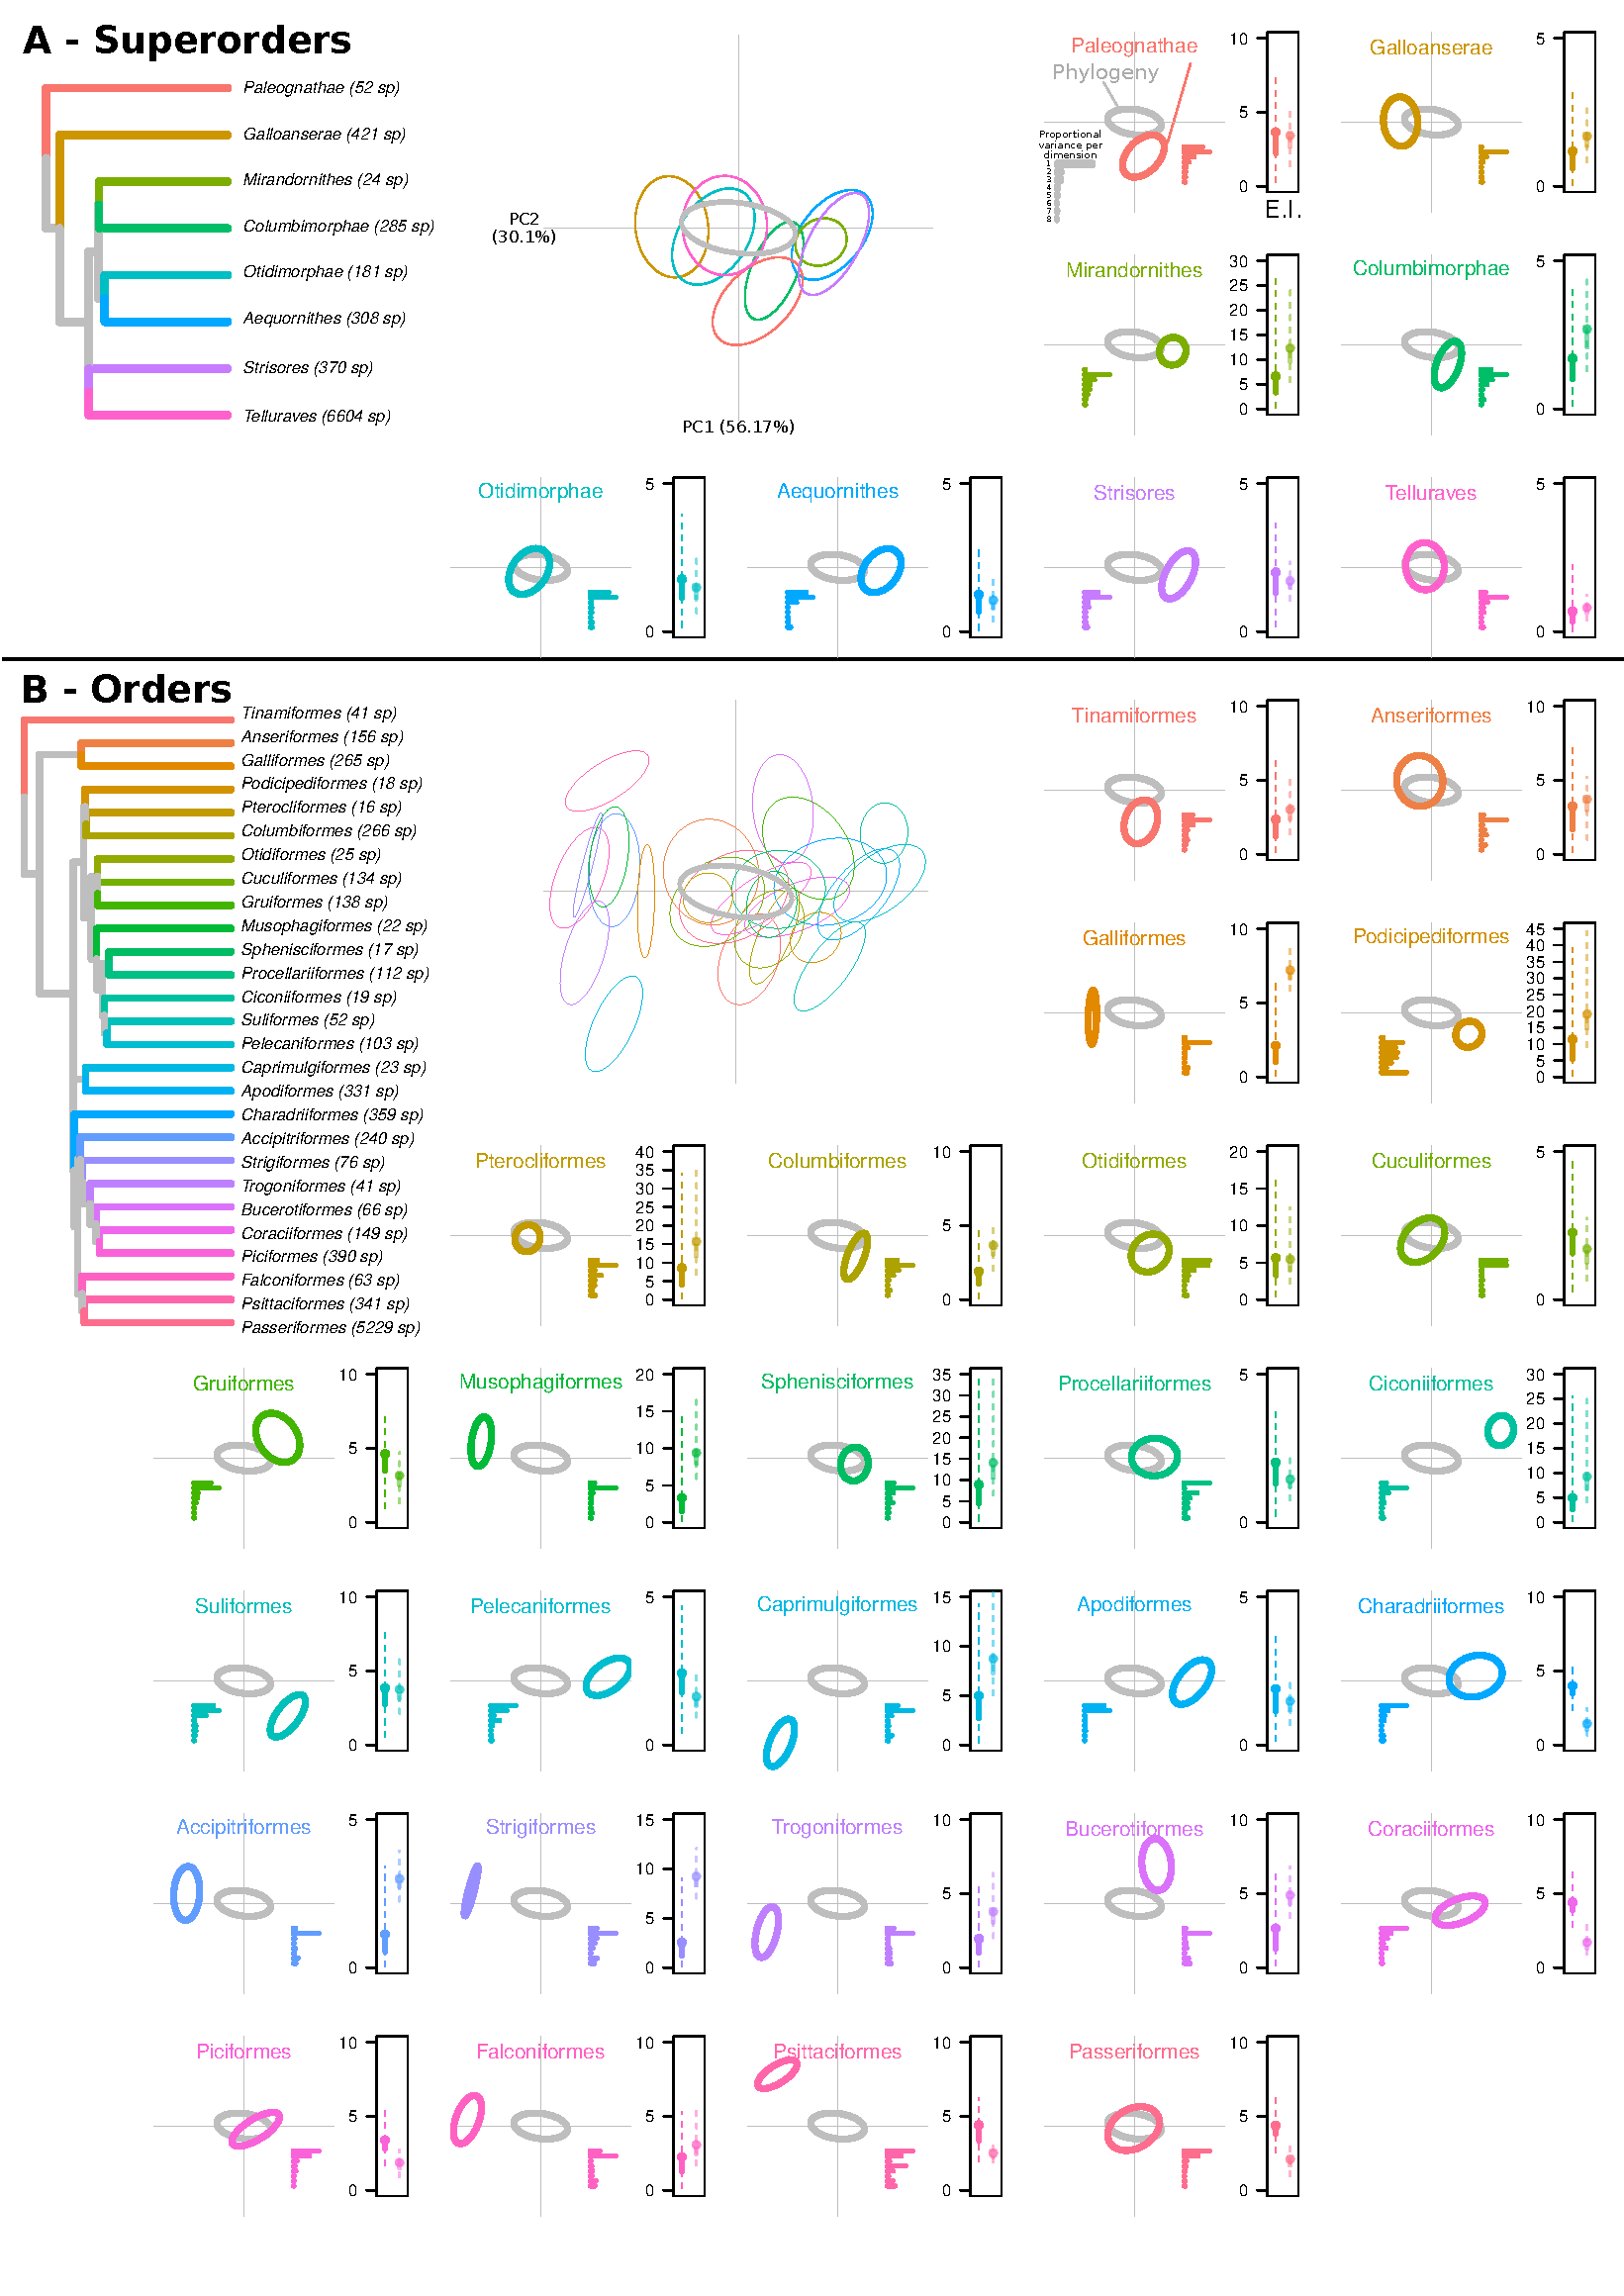
\includegraphics[width=1\textwidth]{Figures/ellipses.pdf}
\caption{.}
\label{Fig:ellipses}
\end{figure}


\begin{figure}[!htbp]
\centering
   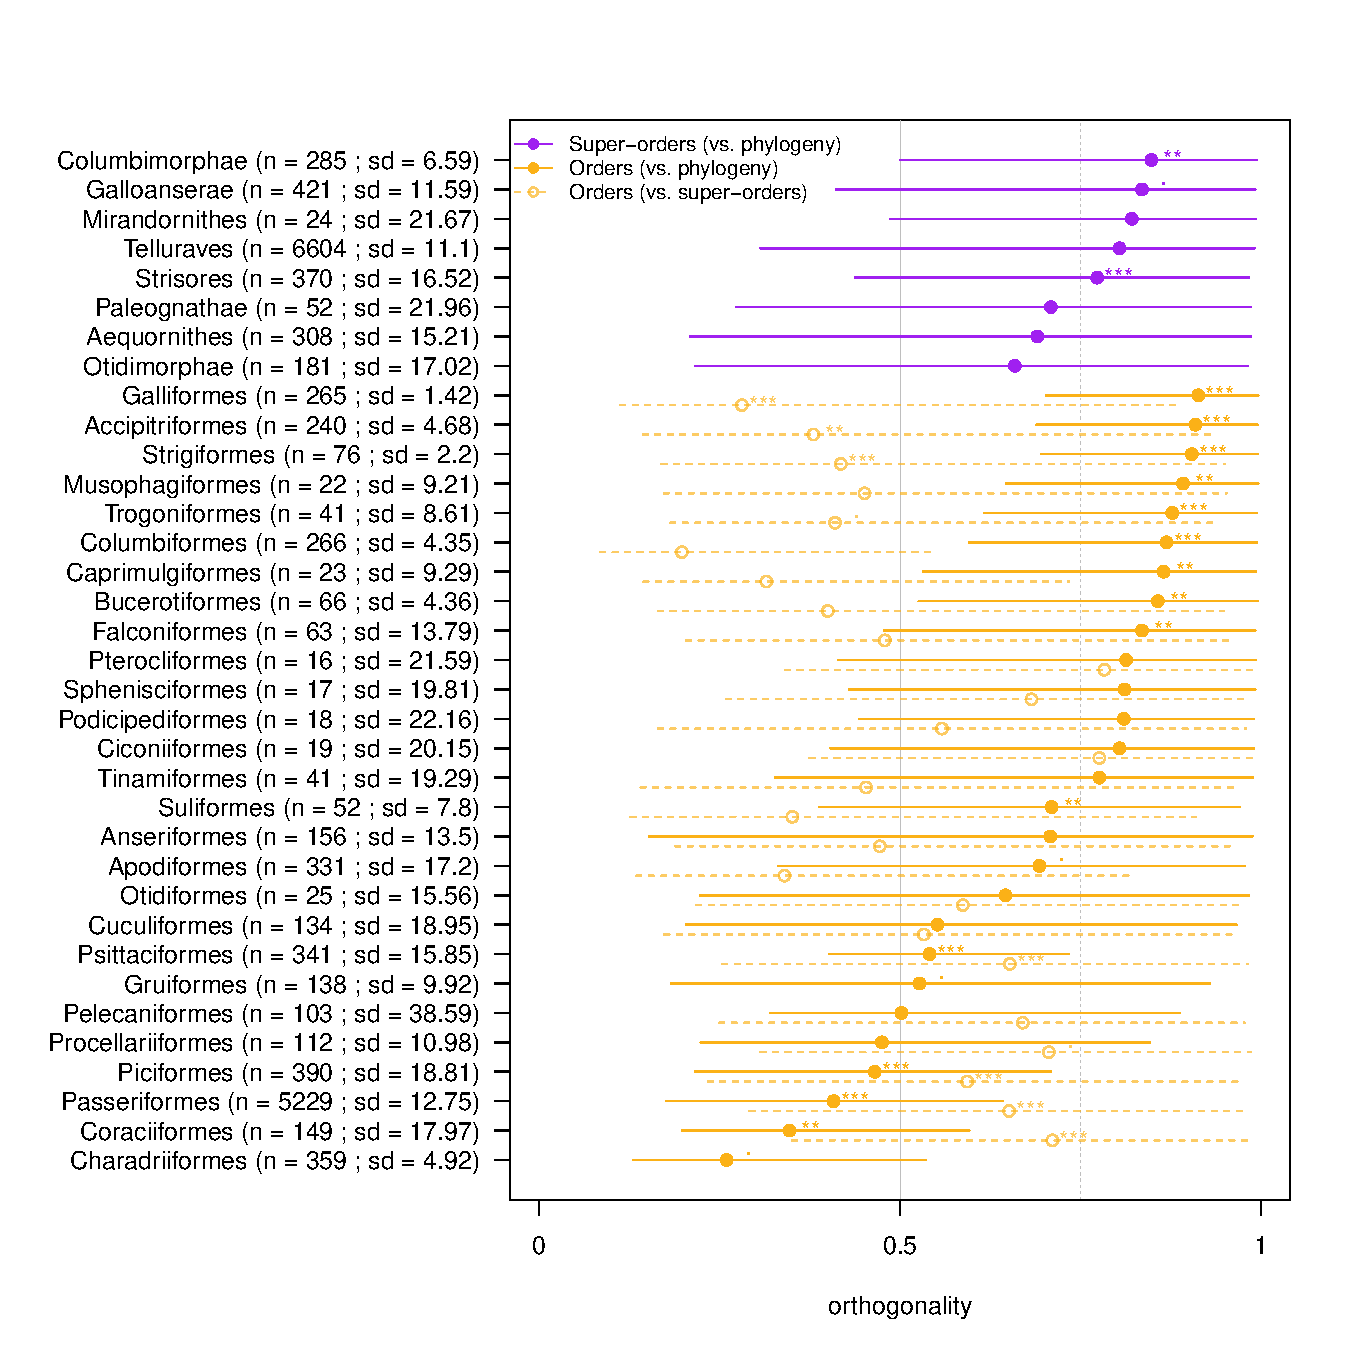
\includegraphics[width=0.9\textwidth]{Figures/orthogonality_results.pdf}
\caption{.}
\label{Fig:orthogonality}
\end{figure}


\begin{figure}[!htbp]
\centering
   % \includegraphics[width=0.9\textwidth]{Figures/phylogenys.pdf}
\caption{.}
\label{Fig:phylogeny}
\end{figure}


\begin{figure}[!htbp]
\centering
   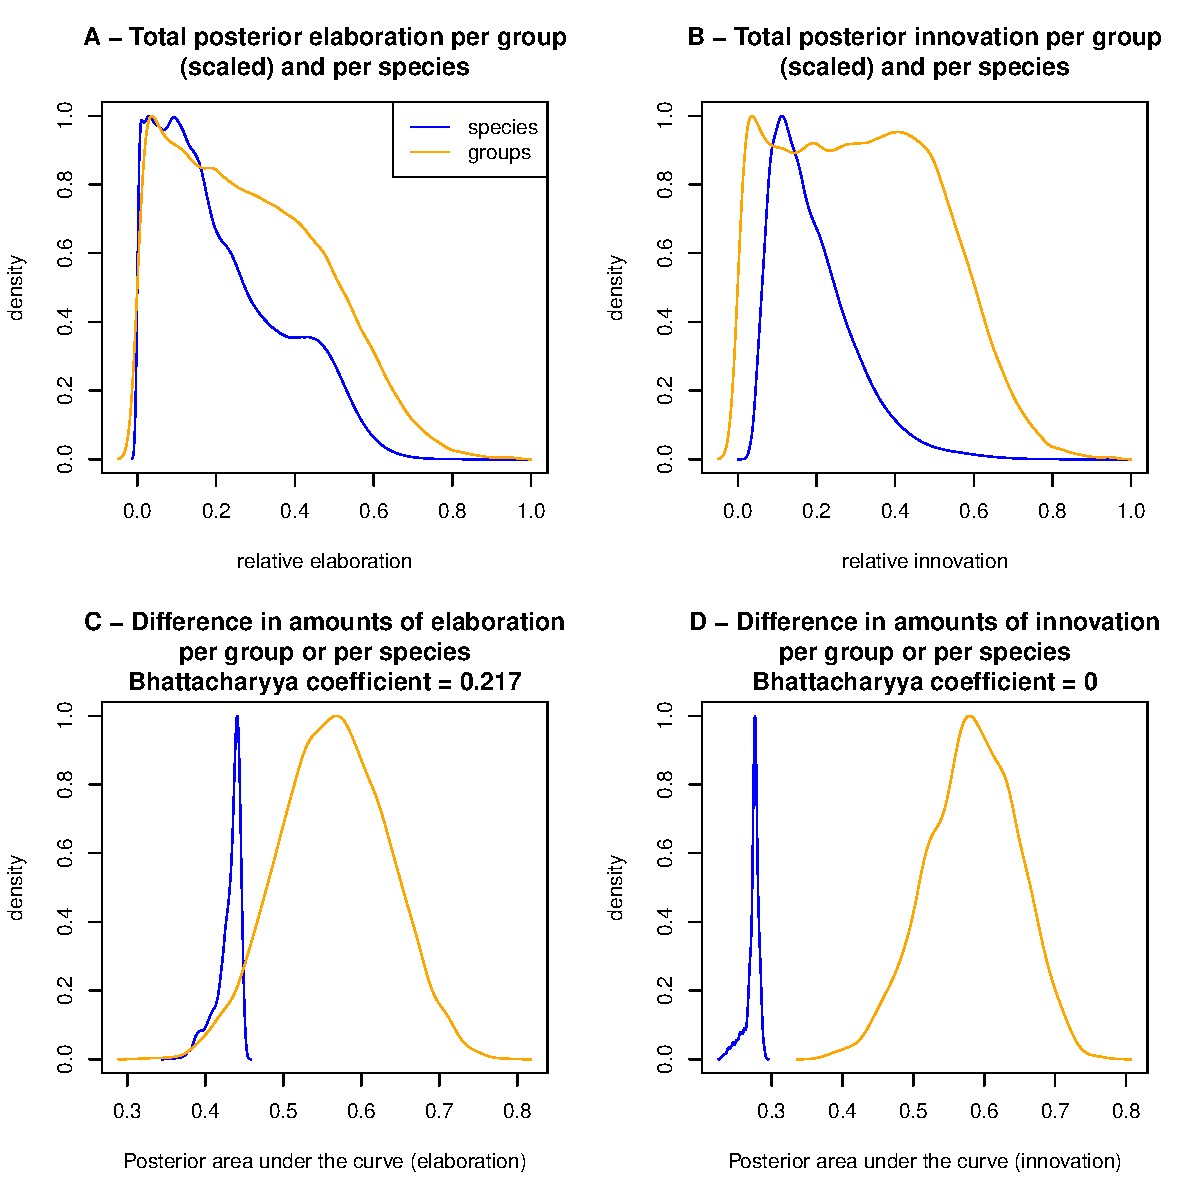
\includegraphics[width=0.9\textwidth]{Figures/relative_EI.pdf}
\caption{.}
\label{Fig:relative_EI}
\end{figure}


\section{Methods}

\bibliographystyle{naturemag}
\bibliography{references}


\end{document}